% ============================================================
%  FR-B4 manuscript — AAMAS 2027 submission
%  Template: official AAMAS 2027 aamas.cls
%  https://warwick.ac.uk/fac/sci/dcs/aamas2027/calls/
%  Compile: pdflatex → bibtex → pdflatex × 2
% ============================================================

%%% For anonymized submission (replace with \documentclass[sigconf]{aamas} for camera-ready)
\documentclass[sigconf,anonymous]{aamas}

% ── AAMAS 2027 copyright block (do not change!) ──────────────
\makeatletter
\gdef\@copyrightpermission{%
  \begin{minipage}{0.2\columnwidth}
   \href{https://creativecommons.org/licenses/by/4.0/}{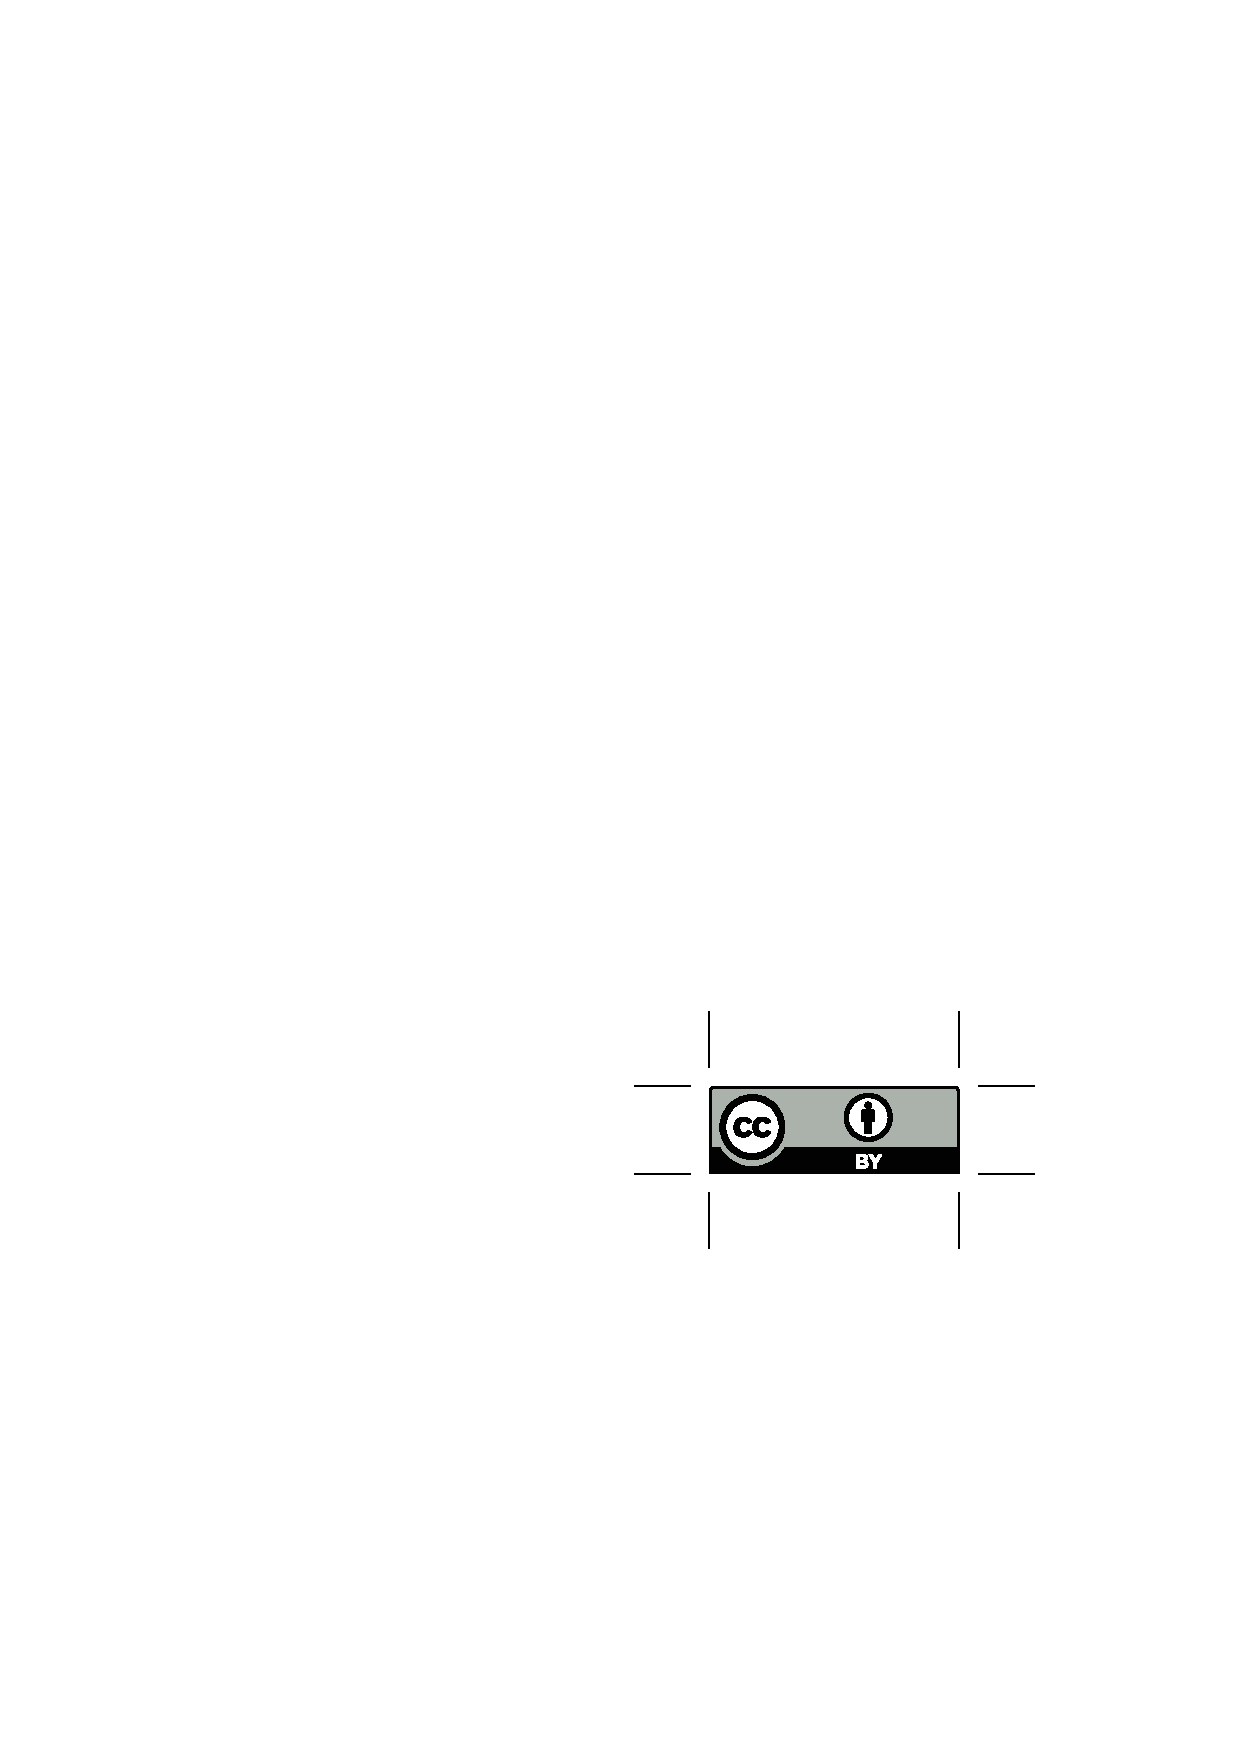
\includegraphics[width=0.90\textwidth]{by}}
  \end{minipage}\hfill
  \begin{minipage}{0.8\columnwidth}
   \href{https://creativecommons.org/licenses/by/4.0/}{This work is licensed under a Creative Commons Attribution International 4.0 License.}
  \end{minipage}
  \vspace{5pt}
}
\makeatother

\setcopyright{ifaamas}
\acmConference[AAMAS 2027]{Proc.\@ of the 26th International Conference
on Autonomous Agents and Multiagent Systems (AAMAS 2027)}{3--7 May 2027}{Hanoi,
Vietnam}{M.~Baldoni, F.~Fang, W.~Yeoh, N.~Yorke-Smith (eds.)}
\copyrightyear{2027}
\acmYear{2027}
\acmDOI{}
\acmISBN{}

\acmSubmissionID{<<OpenReview submission id>>}
\submissionType{Research Paper Track}

% ── Core packages ────────────────────────────────────────────
\usepackage{amsmath,amsthm}
\usepackage{booktabs}
\usepackage{graphicx}
\usepackage{xcolor}
\usepackage{microtype}
\usepackage{balance}        % balanced columns on last page
\usepackage{multirow}
\usepackage{enumitem}


% ── Notation macros ──────────────────────────────────────────
\newcommand{\Dbar}{\bar{\Delta}}
\newcommand{\Lmax}{L_{\max}}
\newcommand{\Lopt}{L_{\mathrm{opt}}}
\newcommand{\Tcorr}{T_{\mathrm{corr}}}
\newcommand{\omdt}{\omega\!\cdot\!dt}
\newcommand{\angbias}{\beta}

% ── AAMAS metadata ───────────────────────────────────────────
\title{When Shared Memory Hurts: Stale-Coordination Failure in\\
       Multi-Agent Particle Collection under a Rotating Latent Field}

\author{Anonymous Authors}
\affiliation{%
  \institution{Anonymous Institution}
  \city{Anonymous City}
  \country{Anonymous Country}}
\email{anonymous@example.org}

\begin{abstract}
Sharing observations across a team of agents improves coordination
under a stationary transport field — but what happens when the
field drifts?  A team that pools a long observation history can
converge confidently on a stale consensus, driving all collectors
toward the wrong direction while independent agents, sampling
noisier but more diverse estimates, collectively cover more ground.
This paper asks where exactly that reversal occurs and what governs it.

Working in a stochastic particle-collection task with a confirmed
stationary coordination benefit ($\Dbar = {+}1.19$ particles,
$n{=}32$ matched seeds), we introduce a linearly rotating field
and measure the last memory window $\Lmax$ that maintains a
statistically significant benefit, across an order-of-magnitude
range of rotation speeds and eight window lengths.

The central finding is evidence for a \emph{stale-coordination failure
mechanism}: the shared arm reduces angular noise but leaves angular
bias unchanged, so beyond a critical window length it drives all
collectors confidently toward a systematically wrong direction,
reducing the inter-agent angular diversity that makes coordination
beneficial.  At both interior speeds ($\omega{\in}\{1.5,5.0\}$), instrumented
runs show the mechanism's predicted directional signatures:
U-shaped shared-arm angular error profiles with observed minima at
their respective $\Lmax$ (paired $t$-tests: $t(31){\geq}3.40$,
$p{<}0.001$ at both speeds), and inter-agent angular dispersion
structurally zero in the shared arm and non-zero in the independent arm.  The coordination benefit landscape under rotation is
\emph{regime-dependent}: qualitatively different outcomes arise at
different rotation speeds.  Four regimes emerge from this study.
A \emph{linear-rotation regime}
($\Lmax/\Tcorr \approx 0.30$, sinc attenuation
negligible) exhibits a clean significance-based crossover at
$\Lmax \approx 0.30\,\Tcorr$ at two interior speeds; a
\emph{sinc-attenuation regime} ($\omega{\in}\{2.0,\,2.5,\,3.0\}$) dampens
the estimate amplitude across the tested $L$ range, suppressing the
sharp crossover; a \emph{rapid-rotation regime} ($\omega{=}10.0$)
drives the predicted $\Lmax$ below integer resolution; and a
\emph{long-episode regime} ($\omega{=}1.0$, $\Tcorr{\approx}H$) exhibits
an unexplained mechanism — raising the question of what governs
which regime a given $(\omega, H)$ pair falls into.
\end{abstract}

\keywords{multi-agent coordination; non-stationary environments;
          memory window; communication benefit; stochastic particle
          collection; rotating latent field}

\begin{CCSXML}
<ccs2012>
  <concept>
    <concept_id>10010147.10010178.10010179.10010182</concept_id>
    <concept_desc>Computing methodologies~Multi-agent planning</concept_desc>
    <concept_significance>500</concept_significance>
  </concept>
  <concept>
    <concept_id>10010147.10010178.10010179</concept_id>
    <concept_desc>Computing methodologies~Cooperative and collaborative learning</concept_desc>
    <concept_significance>300</concept_significance>
  </concept>
</ccs2012>
\end{CCSXML}

\ccsdesc[500]{Computing methodologies~Multi-agent planning}
\ccsdesc[300]{Computing methodologies~Cooperative and collaborative learning}

% ============================================================
\begin{document}
\maketitle
% ============================================================

% ------------------------------------------------------------
\section{Introduction}
\label{sec:intro}
% ------------------------------------------------------------

Communication protocols for multi-agent systems are typically
designed and evaluated against a fixed environment. In deployment,
environments drift.  A team that coordinates on a shared velocity
summary learned under a stationary transport field will
eventually coordinate on a stale estimate as the field rotates,
potentially performing \emph{worse} than if the agents had acted
independently on their own local observations.

This paper asks a precise question: how long must an observation
memory window be to maintain a positive coordination benefit
when the latent transport field rotates at angular rate $\omega$?
We study this in the stochastic particle-collection task of
SPS-C03~\cite{spsC03}, where four mobile collectors must exploit
a weak latent drift $\alpha{=}0.06$ to collect more of $N{=}256$
diffusing particles than a capacity-matched independent team
with no shared information. The confirmed stationary baseline is
$\Dbar{=}{+}1.19$ particles (SD~2.44, $p{<}0.001$, 32 matched
seeds).

We extend this baseline along the temporal axis by introducing
a linearly rotating field $\theta(t) = \theta(0) + \omega \cdot t
\cdot dt$ and asking two implementation-level questions: (i)~what
memory window $L$ should agents use, and (ii)~how does the best
achievable $L$ scale with the rotation rate $\omega$?

\medskip\noindent\textbf{Main result.}
At two interior rotation speeds ($\Tcorr \in \{33, 10\}$),
the pre-registered significance-based threshold satisfies
\[
  \Lmax(\omega) / \Tcorr \approx 0.30, \quad
  \Tcorr = \frac{1}{\omdt},
\]
where $\Tcorr$ is the one-radian decorrelation timescale,
and $\Lmax$ is the significance-based threshold
(Section~\ref{sec:threshold-defs}; two related thresholds, $L^*$
and the coordination-collapse boundary, are defined there).
At these two speeds the empirical ratio $\Lmax/\Tcorr = 0.30$
holds exactly; the window spans $0.27\;\text{rad}$ (slow) and
$0.20\;\text{rad}$ (mid) of total field rotation at the threshold
under the corrected $(L{-}1)$ lag formula — the
\emph{linear-rotation regime} where sinc attenuation is negligible
and the midpoint-lag approximation holds.
Other tested speeds fall into qualitatively different regimes
(see Section~\ref{sec:lmax-scaling}).
The constant $c \approx 0.30$ rests on two interior anchors;
the slow anchor ($p{=}0.049$) was confirmed by a pre-specified
sensitivity analysis at $n{=}64$ ($t{=}{+}1.87$, $p{<}0.05$).
In the slow condition, a window beyond $\Lmax$ reverses the benefit:
$\Dbar$ falls from $+0.94$ at $L{=}10$ to $-0.38$
at $L{=}20$ ($\omega{=}1.5\;\text{rad/step}$).
At mid ($\omega{=}5.0$), the mean $\Dbar$ remains positive until
$L^*{\in}(30,45)$, far beyond $\Lmax{=}3$; a long window can degrade but
does not necessarily reverse the benefit within the tested range.

\medskip\noindent\textbf{Why memory eventually hurts.}
The mechanism is not a degradation of each agent's individual
directional accuracy. Both arms accumulate the same angular lag
($\omega \cdot (L{-}1) \cdot dt/2$ radians at window midpoint); the
shared arm merely reduces angular \emph{noise} while leaving
the bias unchanged. Once the window spans enough rotation, the
shared arm drives all $M$ collectors confidently toward the
same stale direction, eliminating the coverage diversity that
makes independent estimates collectively useful. This is a
policy nonlinearity: the capacity-matching controller maps
confident-but-wrong directions into globally poor coverage.

\medskip\noindent\textbf{Contributions.}
\begin{enumerate}
  \item We provide direct measurement evidence for a stale-coordination
  failure mechanism: at both interior speeds, instrumented runs show
  U-shaped shared-arm angular error with observed minima at their
  respective $\Lmax$, and inter-agent directional dispersion that is
  structurally zero in the shared arm while the independent arm retains
  diversity (Figure~\ref{fig:dispersion}).
  These directional signatures are consistent with the proposed mechanism.
  We do not measure spatial trajectory overlap, spatial coverage directly,
  or provide a formal mediation analysis connecting angular dispersion to
  captures; those remain open.
  \item We identify a four-regime taxonomy of the coordination
  benefit landscape under rotation: (i)~a linear-rotation regime
  ($\omega\Lmax dt \approx 0.30\;\mathrm{rad}$) with a clean
  crossover at $\Lmax/\Tcorr \approx 0.30$; (ii)~a sinc-attenuation
  regime where amplitude damping suppresses the sharp crossover;
  (iii)~a rapid-rotation regime where $\Lmax$ falls below integer
  resolution; and (iv)~a long-episode regime ($\Tcorr{\approx}H$)
  with an unresolved mechanism.
  The $c \approx 0.30$ result is the quantitative finding within
  regime~(i).
  \item We show that the empirical crossover occurs at lower $\Lmax$
  than the bias/noise-parity prediction ($L^* \propto (\omega\,dt)^{-2/3}$),
  a different functional form, attributable to policy nonlinearity.
  \item We show that exponential decay does not follow the
  same $\Lmax \propto \Tcorr$ pattern at the two interior speeds,
  making the sliding window a more tractable choice in the studied regime.
  \item We provide a pre-registered, reproducible experiment with
  event-keyed matched counterfactuals and an explicit reproduction
  gate anchored to SPS-C03.
\end{enumerate}

% ------------------------------------------------------------
\section{Related Work}
\label{sec:related}
% ------------------------------------------------------------

\paragraph{Non-stationary multi-agent environments.}
Non-stationarity in multi-agent settings is usually addressed by
meta-learning or recurrent architectures rather than analytical
memory-length prescriptions~\cite{foerster2018dial,kapturowski2019r2d2}.
These approaches adapt $L$ implicitly through learned gates but
offer no closed-form guidance for practitioners.
Pati\~{n}o et al.~\cite{patino2023turbulent} show that nearest-neighbor
sharing helps aerial swarms compensate for turbulent flows, but
do not derive a staleness threshold.

\paragraph{Windowed and discounted estimation.}
Sliding-window UCB (SW-UCB)~\cite{garivier2011swucb} and
discounted UCB~\cite{kocsis2006discucb} apply the same
bias/variance logic to non-stationary bandit problems:
a window of length $L \approx \sqrt{n/\Delta}$ is near-optimal
under a known breakpoint rate $\Delta$. Our sliding-window controller
is the cooperative analogue of SW-UCB applied to field-direction
estimation across agents. We find a pattern consistent with $1/\omega$ scaling
at two interior rotation speeds ($\Lmax/\Tcorr \approx 0.30$),
steeper than the bias/noise-parity prediction ($L^* \propto \omega^{-2/3}$);
this pattern is preliminary and requires further validation.

\paragraph{Communication under information constraints.}
TarMAC~\cite{das2019tarmac} and IC3Net~\cite{singh2019ic3net}
learn when to suppress messages but do not prescribe a temporal
staleness cutoff. The information-bottleneck approach of
Wang et al.~\cite{wang2020ib} optimises message bandwidth but
not memory depth. Our contribution is orthogonal: we hold the
message fixed (a count-weighted team mean velocity) and vary
only the observation history depth.

\paragraph{Particle collection.}
Wang et al.~\cite{wang2025mobile} establish the single mobile
collector as a benchmark for particle collection in chaotic flows.
Our multi-agent extension isolates whether shared summaries lower
the minimum signal strength needed to exploit a latent field,
and the current paper asks how robustly that benefit persists
under field rotation. The matched-counterfactual design follows
the guidance of Glasserman and Yao~\cite{glasserman1992crn} and
the event-keyed coupling of Buffalo et al.~\cite{buffalo2026ekhash}.

% ------------------------------------------------------------
\section{Model and Theory}
\label{sec:model}
% ------------------------------------------------------------

\subsection{Particle-collection task}

The arena is the unit square $[0,1]^2$ with reflecting boundaries.
$N{=}256$ passive particles diffuse with step size $\sigma{=}0.06$
per \mbox{$dt{=}0.02$} second and are advected by a latent field
with strength~$\alpha{=}0.06$.  Four collectors (sensing radius
$r{=}0.16$, max speed $v_{\max}{=}0.12$) run for $H{=}67$ steps;
a particle is permanently captured when it enters a collector's disc.
The estimand is
\[
  \Delta_s = Y_{\mathrm{shared},s} - Y_{\mathrm{indep},s},
\]
the seed-level difference in unique captures between the
\emph{shared} arm (all agents receive the team mean-velocity
summary) and the \emph{independent} arm (agents use only their
own local observations).

\paragraph{Matched counterfactual coupling.}
Both arms run from the \emph{identical} pre-generated noise tensor
$W_s \in \mathbb{R}^{H \times N \times 2}$, initial particle
positions $X_s^0$, initial collector positions $C_s^0$, and
deterministic field sequence $\theta_s(t)$; only the message
channel differs.  This event-keyed coupling~\citep{buffalo2026ekhash}
ensures that $\Delta_s$ is a within-seed contrast: the stochastic
environment is held constant while communication alone varies.
Equation~\eqref{eq:window} is evaluated over the shared team
history (shared arm) or each agent's own history (independent arm);
all other aspects of the simulation are identical.

\subsection{Rotating-field model}

The latent field direction evolves deterministically:
\[
  \theta(t) = \theta(0) + \omega \cdot t \cdot dt,
  \quad \theta(0) \sim \mathrm{Uniform}[0, 2\pi).
\]
At $\omega{=}0$ the task reduces to SPS-C03 exactly.
The field rotates deterministically, so its cosine similarity
with the current direction oscillates rather than decaying; nonetheless
the one-radian decorrelation timescale—the lag at which cosine similarity
first drops to $\cos(1) \approx 0.54$—is a natural staleness timescale:
\[
  \Tcorr = \frac{1}{\omdt} \quad (\text{steps}).
\]
Note the $dt$ factor: it is the \emph{per-step} rotation
$\omdt$, not the rate $\omega$ itself, that determines how
quickly observations become stale.

\paragraph{Threshold definitions.}
\label{sec:threshold-defs}
Three distinct $L$-based thresholds appear in the results;
they coincide only under specific conditions:
\begin{itemize}[noitemsep,topsep=2pt]
  \item \emph{Significance threshold} ($\Lmax$): the largest $L$
        at which the pre-registered one-sided $t$-test gives $p{<}0.05$.
        This is a statistical-detectability threshold,
        not a behavioural reversal.
  \item \emph{Zero-crossing threshold} ($L^*$): the value of $L$ at
        which $\mathbb{E}[\Delta]$ changes sign, estimated by
        interpolation between adjacent grid points.
  \item \emph{Coordination-collapse boundary}: the $L$ at which the
        expected captures under the shared arm fall below the
        independent arm — equivalent to the zero-crossing.  We use
        this phrase only when $\Lmax \approx L^*$, i.e.\ when the
        significance threshold and the sign reversal are in the same
        $L$-interval.
\end{itemize}

\subsection{Memory controllers}

\paragraph{Sliding-window controller (window).}
At step $t$, agent $i$ computes the count-weighted mean velocity
from the last $L$ steps of all agents' observations (shared arm)
or its own (independent arm):
\begin{equation}
  \hat{v}(t, L) =
  \frac{\sum_{\tau=\max(0,t-L+1)}^{t}
        \sum_i n_i(\tau)\,\bar{v}_i(\tau)}
       {\sum_{\tau}\sum_i n_i(\tau)},
  \label{eq:window}
\end{equation}
where $n_i(\tau)$ is the count of particles observed by agent $i$
at step $\tau$ and $\bar{v}_i(\tau)$ is their local mean velocity.
At $L{=}H$ this reduces to the full-episode SPS-C03 controller.

\paragraph{Capacity-matching action rule.}
The estimated velocity $\hat{v}$ is converted to a movement
command by the capacity-matching blend:
\begin{equation}
  a_m = \mathrm{unit}\!\bigl(w_t\,\hat{f} + (1-w_t)\,\hat{d}_m\bigr),
  \qquad
  \hat{f} = -\mathrm{unit}(\hat{v}),
  \label{eq:action}
\end{equation}
where $\hat{d}_m = \mathrm{unit}(\bar{p}_m)$ is the unit vector toward
agent $m$'s local particle centroid, $\bar{p}_m$ is the mean relative
position of visible particles, $N_{\max}$ is the per-agent sensing
capacity (particles per step at full-disc occupancy), and the blend
weight $w_t = \min(0.7,\,2\,\bar{n}_t/N_{\max})$ rises with the current
mean per-agent particle count $\bar{n}_t$ (instantaneous, at step $t$).
When $\hat{v}{=}0$ (no observations in the window), agents fall back
to the density term alone.
All agents in the shared arm receive the same $\hat{v}$ and hence
the same $\hat{f}$; they differ only in $\hat{d}_m$.  The policy
nonlinearity arises here: a high blend weight $w_t$ causes all
collectors to commit strongly to $\hat{f}$, so a stale $\hat{v}$
drives the entire team toward a single wrong direction, eliminating
the diversity in $\hat{d}_m$ that would otherwise provide spatial
coverage.

\paragraph{Exponential-decay controller (decay).}
The same sum with exponentially decreasing weights
$\lambda^{t - \tau}$, $\lambda{=}\exp(-1/L)$. The effective
memory length equals $L$ in expectation, but older observations
are downweighted smoothly rather than discarded at a hard cutoff.

\subsection{Signal-to-noise analysis and its limits}
\label{sec:theory-fail}

A natural first hypothesis is that sharing $M$ agents' observations
improves the effective sample size by $M$, giving a
signal-to-noise ratio
$\mathrm{SNR}_{\mathrm{shared}}/\mathrm{SNR}_{\mathrm{indep}} = \sqrt{M}$
independent of $L$ and $\omega$.  If field performance were linear
in SNR, coordination would help at every $L$ — yet $\Dbar$ goes
negative at large $L$.  The model misses a crucial asymmetry:
\emph{sharing reduces angular noise but not angular bias}.

Define the angular bias (lag to the window midpoint),
\[
  \angbias(L,\omega) = \frac{\omega \cdot (L-1) \cdot dt}{2}
    \quad \text{(radians)},
\]
and the angular noise of the shared arm,
\[
  \sigma_{\theta,\mathrm{shared}}(L) =
  \frac{\sigma}{\alpha\sqrt{M\bar{K} L\, dt}},
\]
where $\bar{K} = \mathbb{E}_t[\bar{n}_t]$ is the mean per-agent particle
count averaged over steps (the episode mean of the instantaneous
count $\bar{n}_t$ used in the action rule; $\bar{K}{\approx}8$ at
the studied parameters).
Both arms carry the same bias $\angbias$; sharing only reduces
$\sigma_\theta$ by $\sqrt{M}$.  As $L$ grows, the shared arm's
direction estimate becomes increasingly \emph{precise around the
wrong direction}: it drives all $M$ collectors confidently toward
$\hat{\theta} = \theta(t) - \angbias$.  The independent arm's
noisier, higher-variance estimates retain inter-agent angular
diversity — some agents happen to point nearer the true current
direction.  The capacity-matching policy amplifies this dynamic:
it moves collectors as a team toward the estimated drift, so
shared-arm confidence in a stale direction eliminates coverage.

The bias/noise-parity threshold ($\angbias \approx
\sigma_{\theta,\mathrm{shared}}$) gives $L^* \propto (\omega\,dt)^{-2/3}$.
This is a different functional form from the empirical
$\Lmax \propto (\omega\,dt)^{-1}$: the ratio $L^*/\Tcorr$
scales as $(\omega\,dt)^{1/3}$ and is therefore not a universal
constant.  Because the actual threshold is set by the
\emph{policy}'s nonlinear sensitivity rather than directional MSE,
the empirical crossover is earlier and follows a steeper scaling.

\begin{table}[t]
\centering
\caption{Angular bias and shared-arm noise at and beyond
$\Lmax$.  At $L{=}\Lmax$ the bias is well below
$\sigma_{\theta,\mathrm{shared}}$; the ratio first exceeds 1 at
approximately $2\Lmax$, consistent with a policy-driven crossover
at lower $L$ than the directional-MSE model predicts.}
\label{tab:bias-noise}
\setlength\tabcolsep{5pt}
\begin{tabular}{lrrrr}
\toprule
$\omega\;(\Tcorr)$ & $L$ & $\omega(L{-}1)dt$ & $\angbias$ & $\angbias/\sigma_{\theta,\mathrm{shared}}$\\
\midrule
$1.5\;(33)$ & 10 (=$\Lmax$) & 0.27 rad & 0.135 rad & 0.34 \\
$1.5\;(33)$ & 20            & 0.57 rad & 0.285 rad & 1.02 \\
$5.0\;(10)$ &  3 (=$\Lmax$) & 0.20 rad & 0.100 rad & 0.14 \\
$5.0\;(10)$ & 10            & 0.90 rad & 0.450 rad & 1.14 \\
\bottomrule
\end{tabular}
{\small ($\alpha{=}0.06,\;\sigma{=}0.06,\;M{=}4,\;dt{=}0.02$;
$\bar{K}{\approx}8$ is the episode-mean per-agent particle count
defined in Section~\ref{sec:theory-fail})}
\end{table}

\medskip
\noindent\textbf{Regime structure of the window estimate.}
The midpoint-lag formula $\hat\theta = \theta(t) - \omega(L{-}1)\,dt/2$
(and the bias/noise analysis above) is valid only when
$\omega L\,dt \ll 1$, i.e.\ when the window spans a small total
rotation.  Beyond this linear-rotation regime, the window estimate
is governed by the exact geometric-sum formula in
Appendix~\ref{app:theory}, whose amplitude scales as
$|\sin(\omega L\,dt/2)|/(L|\sin(\omega\,dt/2)|)$.  Two
qualitatively distinct failure modes result:
\begin{enumerate}
  \item \emph{Sinc-attenuation regime.}  When $\omega L\,dt$ is
  substantial but the amplitude is still positive,
  both the noise-reduction benefit and the stale-direction cost
  are scaled down together.  The mechanism operates but weakly,
  producing gradual degradation rather than a sharp crossover.
  \item \emph{Rapid-rotation regime.}  When $\Tcorr$ is so short
  that $c\,\Tcorr < 1$ step (predicted $\Lmax < 1$), no
  integer-valued $L$ lies inside the linear-rotation regime.
  Even $L{=}1$ carries a per-step rotation $\omega\,dt$ as its
  lag angle, and the resulting benefit is too small to detect at
  practical sample sizes.
\end{enumerate}
A third anomaly at very slow rotation ($\omega{=}1.0$,
$\Tcorr{\approx}H$) lies outside both accounts; its mechanism
is not resolved in this work.  Section~\ref{sec:lmax-scaling}
characterises all four regimes empirically.

% ------------------------------------------------------------
\section{Experimental Setup}
\label{sec:setup}
% ------------------------------------------------------------

\subsection{Grid design}

We test four non-stationary rotation speeds and one stationary
baseline, plus a supplementary third-anchor condition ($\omega{=}2.5$,
between slow and mid), eight $L$ levels, and two methods:

\smallskip
\begin{center}
\setlength\tabcolsep{4pt}
\begin{tabular}{llrr}
\toprule
Label & $\omega$ (rad/step) & $\omdt$ & $\Tcorr$ \\
\midrule
stationary & 0    & 0     & $\infty$ \\
very\_slow & 0.75 & 0.015 & 67       \\
slow       & 1.5  & 0.030 & 33       \\
\textit{supp.} & \textit{2.5}  & \textit{0.050} & \textit{20} \\
mid        & 5.0  & 0.100 & 10       \\
fast       & 17.0 & 0.340 & 3        \\
\bottomrule
\end{tabular}
\end{center}

\smallskip\noindent
$L$ levels: $\{1, 3, 5, 10, 20, 30, 45, 67\}$ steps; methods:
sliding window and exponential decay.
The primary design yields 40 active conditions (4 non-stationary
$\omega \times 5$ primary $L \times 2$ methods), plus 24
intermediate-$L$ cells for slow and mid, plus stationary-$\omega$
cells, and 16 supplementary cells for the $\omega{=}2.5$ anchor
(8 $L$ levels $\times$ 1 method — window only).
We call slow and mid the \emph{interior} rotation speeds: they are
the two conditions where $\Lmax$ falls strictly within the grid
range $(1, H)$ and the linear-rotation regime ($\omega\Lmax dt
\lesssim 0.30\;\text{rad}$) applies.  Intermediate $L$ values were
concentrated at these interior speeds (slow, mid, $\omega{=}2.5$) by
design: very\_slow has $\Lmax{=}67$ (boundary, unresolvable within
the grid) and fast has predicted $\Lmax{<}1$ step (below grid
resolution).
Post-hoc exploratory runs at $\omega{=}1.0$ ($\Tcorr{=}50$) and
$\omega{=}2.0$ ($\Tcorr{=}25$), each 8 $L$ levels $\times$ 32 seeds
(window method), are reported in Sec.~\ref{sec:lmax-scaling}.

\subsection{Matched counterfactuals}

Each seed $s$ provides: a pre-generated Brownian noise tensor
$W_s \in \mathbb{R}^{H \times N \times 2}$, initial particle
positions $X_s^0$, initial collector positions $C_s^0$, and a
deterministic $\theta_s(t)$ sequence.  The shared and independent
arms run \emph{from the same tensor}; only the message channel
differs.  This follows the event-keyed coupling of
\citet{buffalo2026ekhash}.

\subsection{Seeds and statistical power}

Seeds 9001--9032 (32 per cell) provide SE $\approx 0.45$ per cell
(SD~$\approx 2.5$), sufficient to detect $|\Dbar| \approx 0.9$
at 80\% power one-sided.  The stationary condition uses seeds
6001--6128 (128 per cell) to resolve the smaller $L$-dependent
effect at $\omega{=}0$.

\subsection{Reproduction gate}

Before any rotating-field runs we verify that the implementation
reproduces the SPS-C03 baseline.  Gate criterion:
$\omega{=}0$, $L{=}1$ (stateless window), seeds 6001--6032:
$\Dbar \in [+0.69, +1.69]$, sign count $\geq 20/32$.

\textbf{Gate result:} $\Dbar{=}{+}1.188$ (SE${}=0.213$),
sign${=}20/32$.  One-sided $t$-test (same test used for all
$\Lmax$ cells): $t{=}5.58$, $df{=}31$, $p{<}0.001$.
Both gate criteria satisfied. \checkmark

\subsection{Pre-registered analysis}

Primary: one-sided $t$-test per cell ($H_0: \Delta \leq 0$,
$\alpha_{\mathrm{test}}{=}0.05$).  $\Lmax(\omega)$ is the largest
$L$ with $p{<}0.05$ for the window method.  Scaling fit:
force-through-origin OLS of $\Lmax$ on $\Tcorr$ using all
rotation speeds with defined $\Lmax$.

% ------------------------------------------------------------
\section{Results}
\label{sec:results}
% ------------------------------------------------------------

\noindent Recall the three threshold types defined in
Section~\ref{sec:threshold-defs}: significance threshold ($\Lmax$),
zero-crossing ($L^*$), and coordination-collapse boundary.
Applied to the current data:
for the slow condition ($\omega{=}1.5$), $\Lmax{=}10$ and
$L^*{\in}(10,20)$ are in the same interval, making $\Lmax$ an
approximate coordination-collapse boundary.
For the mid condition ($\omega{=}5.0$), $\Lmax{=}3$ but
$L^*{\in}(30,45)$: $\Lmax$ marks only statistical detectability;
mid does not exhibit a coordination-collapse boundary within the
tested grid.

\subsection{Per-cell coordination benefit}

Table~\ref{tab:main} shows $\Dbar$, SE, and significance for
all window-method cells. The stationary condition ($\omega{=}0$)
gives significant benefit at $L \in \{1, 3, 10\}$ but not at
$L{=}30$, consistent with the stationary controller's own
optimal window (pooling over a full episode loses little given
$\Dbar$ is nearly flat at $L{\leq}10$).

For $\omega{=}\text{slow}$ ($\Tcorr{=}33$) the coordination
benefit is large and positive for $L \leq 10$ and sharply
negative for $L \geq 20$:
$\Dbar$ goes from $+0.94$ ($L{=}10$, $p{=}0.049$) to
$-0.38$ ($L{=}20$, $p{=}0.79$), a swing of $>1.3$ particles
when the window doubles from 10 to 20 steps.

For $\omega{=}\text{mid}$ ($\Tcorr{=}10$) significance is lost
earlier but the character differs from slow: $\Dbar{=}{+}0.91$ at
$L{=}3$ ($p{=}0.004$) falls to $+0.22$ at $L{=}5$ (NS) and the
estimated mean remains positive through $L{=}30$.  The mean does
not turn negative until $L{=}45$ ($\Dbar{=}{-}0.25$).  The mid
condition therefore primarily demonstrates \emph{loss of detectable
advantage} at $L{>}3$, not the sharp sign reversal seen in slow.

For $\omega{=}\text{fast}$ ($\Tcorr{=}3$) no $L$ value achieves
consistent significance.  The isolated $p{=}0.023$ at $L{=}5$
is an outlier: adjacent cells $L{\in}\{1,3,10\}$ are all
non-significant.  As additional post-hoc analysis (not required
by the pre-registered per-cell criterion), applying Holm's
step-down procedure across the 24 fast cells yields an adjusted
$p_{\mathrm{adj}} = 0.023 \times 24 = 0.55$ for the minimum
raw $p$, confirming no fast cell survives even relaxed correction.
Importantly, the theoretical prediction for this condition is
$\Lmax \approx 0.30 \times 3 = 0.9$ steps, which falls \emph{below}
the minimum grid value of $L{=}1$.  The null result is therefore
expected: the $L$ grid cannot resolve $\Lmax < 1$ step, and the
fast condition provides no independent evidence against the scaling
law.

A supplementary condition $\omega{=}2.5$ ($\Tcorr{=}20$ steps,
between slow and mid) was run with 32~seeds across all 8~$L$~levels
to probe the scaling at an intermediate rotation speed.  $\Dbar$
remains positive at every~$L$ (range $+0.69$ to $+1.72$), with a
local minimum of $+0.78$ at $L{=}10$ ($t{=}1.91$).  The one-sided
$t$-test is significant ($p{<}0.05$) at every $L$ through $L{=}45$
($t{=}1.86$) but not at $L{=}67$ ($t{=}1.67$); no crossover to
negative $\Dbar$ was observed.  The interpretation of $\Lmax$ for
this condition is discussed in Section~\ref{sec:lmax-scaling}.

\begin{table*}[t]
\centering
\caption{Window-method per-cell results.
         $n{=}32$ seeds per cell (non-stationary $\omega$);
         $n{=}128$ for stationary $L{\in}\{1,3,10,30\}$.
         $\Dbar$ = mean shared$-$independent captures;
         ($*$) = $p{<}0.05$ one-sided $t$-test.
         Dashes: intermediate $L$ not run for that $\omega$.
         $\dagger$Stationary $L{=}67$: full-history ($L{=}H$)
         sliding-window cell included for comparison ($n{=}8$ seeds).
         The SPS-C03 baseline ($\Dbar{=}{+}1.19$) is reproduced
         by the $\omega{=}0$, $L{=}1$ reproduction gate
         (Section~\ref{sec:setup}, App.~\ref{app:gate}); the $L{=}67$
         stationary cell coincidentally yields the same value;
         field stationarity removes temporal bias, reducing but not
         eliminating the effect of window length on estimator variance.
         $\omega{=}2.5$: supplementary condition; see Sec.~\ref{sec:lmax-scaling}.
         Exploratory conditions $\omega{\in}\{1.0,\,2.0,\,3.0,\,10.0\}$
         are not included here; their $\Lmax$ values appear in
         Table~\ref{tab:lmax} and their $t$-profiles are
         discussed in Sec.~\ref{sec:lmax-scaling}.}
\label{tab:main}
\setlength\tabcolsep{5pt}
\begin{tabular}{lrrrrrrrr}
\toprule
$\omega\;(\Tcorr)$
  & $L{=}1$ & $L{=}3$ & $L{=}5$ & $L{=}10$
  & $L{=}20$ & $L{=}30$ & $L{=}45$ & $L{=}67$ \\
\midrule
$0\;(\infty)$
  & $+1.19^*$ & $+0.81^*$ & --- & $+0.72^*$
  & --- & $+0.25$ & --- & $+1.19^{*\dagger}$ \\
$0.75\;(67)$
  & $+0.53$ & $+0.47$ & $+0.06$ & $+0.22$
  & $+0.50$ & $+0.41$ & $+0.66$ & $+0.78^*$ \\
$1.5\;(33)$
  & $+1.47^*$ & $+1.50^*$ & $+1.66^*$ & $+0.94^*$
  & $-0.38$ & $-0.28$ & $-0.47$ & $-0.44$ \\
$2.5\;(20)$
  & $+1.72^*$ & $+1.47^*$ & $+1.19^*$ & $+0.78^*$
  & $+1.06^*$ & $+0.88^*$ & $+0.88^*$ & $+0.69$ \\
$5.0\;(10)$
  & $+0.88^*$ & $+0.91^*$ & $+0.22$ & $+0.25$
  & $+0.56$ & $+0.16$ & $-0.25$ & $+0.03$ \\
$17.0\;(3)$
  & $+0.47$ & $+0.47$ & $+0.78$ & $-0.09$
  & $+0.09$ & $-0.38$ & $+0.13$ & $+0.25$ \\
\bottomrule
\end{tabular}
\end{table*}

\subsection{$\Lmax$ versus $\Tcorr$}
\label{sec:lmax-scaling}

Table~\ref{tab:lmax} summarises $\Lmax$ (last significant $L$
under the pre-registered per-cell $p{<}0.05$ criterion,
window method) per rotation speed and the ratio $\Lmax/\Tcorr$.
An alternative operationalisation is the zero-crossing $L^*$
where $\Dbar$ first turns negative: for slow, $L^* \in (10, 20)$
(sign change between adjacent grid values); for mid, $L^* \in (30, 45)$.
At slow, $\Lmax$ and $L^*$ approximately agree (both locate the crossover
near $L{=}10$--$20$): the significance threshold and the zero-crossing
are close, consistent with a genuine coordination-collapse boundary
in that range.
At mid, however, $\Lmax{=}3$ while $L^*{\in}(30, 45)$ —
a tenfold gap.  $\Dbar$ remains positive at $+0.22$ through $L{=}30$
and only turns negative at $L{=}45$; $\Lmax{=}3$ therefore marks
\emph{loss of statistical detectability} rather than a coordination-collapse
boundary.  Under the zero-crossing operationalisation, mid gives
$c^* \in (3.0, 4.5)$ — an order of magnitude above the significance-based
$c{=}0.30$.  The $c{=}0.30$ result is therefore primarily anchored on
the slow condition where the two operationalisations agree; mid corroborates
the $1/\Tcorr$ scaling pattern for $\Lmax$ but measures a different
crossover quantity at the same $\Lmax$ value.  The significance-based
$\Lmax$ is used throughout as the pre-registered quantity.

\begin{table}[b]
\centering
\caption{$\Lmax$ (last $L$ with $p{<}0.05$, window) and
         ratio to $\Tcorr$, with regime label.
         Bold: two clean interior points (slow, mid)
         in the linear-rotation regime with $\Lmax/\Tcorr = 0.30$.
         $\P\;\omega{=}1.0$: only $L{=}1$ significant ($t{=}2.68$);
         all $L{\geq}3$ non-significant ($t{<}0.5$).
         $\S\;\omega{=}2.5$: $\Lmax{=}45$ by criterion ($t{=}1.86$),
         but $t$-profile non-monotone (sinc-attenuation regime).
         $\ddagger\;\omega{=}2.0$: all $L$ significant throughout;
         $\Lmax$ is a lower bound (${\geq}67$; sinc-attenuation).
         $\dagger\;\omega{=}10.0$: only $L{=}30$ significant ($t{=}2.04$),
         but estimate amplitude is 4.7\% at $L{=}30$ (near-zero
         cancellation); likely false positive — see text.
         $\|\;\omega{=}3.0$: $n{=}64$; $L{=}5$ significant ($t{=}2.57$) as
         predicted, but benefit persists through $L{=}67$ ($t{=}2.86$);
         sinc-attenuation regime, $\Lmax$ is a lower bound.}
\label{tab:lmax}
\setlength\tabcolsep{4pt}
\begin{tabular}{lrrrrl}
\toprule
$\omega$ & $\Tcorr$ & $\Lmax$ & $\omega\Lmax dt$ & $\Lmax/\Tcorr$ & Regime \\
\midrule
0.75 & 67 & 67            & 1.00 rad          & 1.00 & linear (bdy.) \\
1.0  & 50 & 1$^{\P}$     & 0.02 rad          & 0.02 & long-ep. \\
1.5  & 33 & 10            & \textbf{0.30 rad} & \textbf{0.30} & \textbf{linear} \\
2.0  & 25 & ${\geq}$67$^{\ddagger}$ & ${\geq}$2.68 rad & ${\geq}$2.68 & sinc-att. \\
2.5  & 20 & 45$^{\S}$    & 2.25 rad          & 2.25 & sinc-att. \\
3.0  & 17 & ${\geq}$67$^{\|}$ & ${\geq}$4.02 rad & ${\geq}$4.02 & sinc-att. \\
5.0  & 10 &  3            & \textbf{0.30 rad} & \textbf{0.30} & \textbf{linear} \\
10.0 &  5 & ---$^{\dagger}$ & ---            & ---  & rapid-rot. \\
17.0 &  3 & ---           & ---               & --- & rapid-rot. \\
\bottomrule
\end{tabular}
\end{table}

\noindent
The two interior rotation speeds (slow and mid) give exactly
$\Lmax/\Tcorr = 0.30$.  The very\_slow condition ($\Tcorr{=}67$)
gives $\Lmax{=}67$ — the full episode — which is consistent with
the $1/\omega$ scaling but does not sharpen the constant because any
true $\Lmax$ between 45 and 67 would produce the same reported
value within our $L$ grid.  The fast condition ($\Tcorr{=}3$)
has no reliable $\Lmax$.

The supplementary condition $\omega{=}2.5$ ($\Tcorr{=}20$, predicted
$\Lmax\approx6$) was run with 32~seeds to test whether $c{=}0.30$
holds at an intermediate rotation speed.  Applying the same
pre-registered criterion used for slow and mid (last $L$ with one-sided
$t$-test $p{<}0.05$, $n{=}32$), we obtain $\Lmax(\omega{=}2.5){=}45$
($t{=}1.86$, $p{<}0.05$); $L{=}67$ falls below threshold
($t{=}1.67$, $p{>}0.05$).  This gives $c{=}45/20{=}2.25$ —
$7.5\times$ above the two-anchor value.  However, the $t$-profile is
\emph{non-monotone}: after peaking at $L{=}1$ ($t{=}3.07$) it dips
at $L{=}10$ ($t{=}1.91$), recovers at $L{=}20$ ($t{=}2.38$) and
$L{=}30$ ($t{=}1.97$), then declines through $L{=}45$ ($t{=}1.86$)
to $L{=}67$ ($t{=}1.67$).  A genuine sharp crossover — as at slow,
where $\Dbar$ drops from $+0.94$ to $-0.38$ across a single $L$
doubling — produces a monotone decline and a clear sign reversal; the
$\omega{=}2.5$ profile shows neither.  The $\omega{=}2.5$ condition
therefore \emph{cannot serve as a clean third anchor}: the stopping
criterion delivers a technical $\Lmax{=}45$, but not a genuine sharp
crossover.  \textbf{The headline $c \approx 0.30$
continues to rest on the two interior anchor points (slow, mid).}
We report it as a preliminary value; the $\omega{=}2.5$ result
suggests that the true relationship may be more complex — in
particular, that the crossover sharpness itself depends on $\omega$.

An exploratory run at $\omega{=}2.0$ ($\Tcorr{=}25$, predicted
$\Lmax\approx7.5$) with 32~seeds (window method) reveals a second
broad-benefit anomaly: the one-sided $t$-test is significant at
every $L$ in the grid, with $t$-statistics ranging from $t{=}5.57$
at $L{=}1$ to a minimum of $t{=}1.93$ at $L{=}45$, and recovering
to $t{=}2.07$ at $L{=}67$ ($p{<}0.05$ throughout).  The full-episode
$L{=}67$ window remains beneficial, giving $\Lmax\geq67$
($c\geq67/25{=}2.68$) — a lower bound.  Like $\omega{=}2.5$,
this condition does not yield a genuine crossover and cannot serve
as an anchor.

An exploratory run at $\omega{=}10.0$ ($\Tcorr{=}5$, predicted
$\Lmax \approx 1.5$ under $c{=}0.30$) with 32~seeds reveals the
\emph{rapid-rotation regime}.  The only nominally significant cell
is $L{=}30$ ($t{=}2.04$, $p{<}0.05$), but this result should not
be taken as a real coordination benefit.  At $L{=}30$ the window
estimate amplitude — computed from the geometric-sum formula in
Appendix~\ref{app:theory} — is only $4.7\%$ of the single-step
amplitude ($\approx 0.047$ from the geometric-sum formula):
near-zero cancellation, the window spanning nearly one full
rotation ($\omega L\,dt{=}6.0\;\text{rad} \approx 2\pi$).  The estimate direction is $-166^\circ$
relative to the current field — nearly backwards — with
negligible amplitude.  An estimate of this quality cannot explain
a genuine coordination benefit; the $t{=}2.04$ result is consistent
with the expected $0.4$ false positives from testing eight $L$
cells at $\alpha{=}0.05$.
The $L$ values flanking the anomaly confirm the diagnosis:
at $L{=}1$ (the predicted $\Lmax$ at $c{=}0.30$), the estimate
is accurate (magnitude~1.0, $0^\circ$ lag), yet the benefit is
not significant ($t{=}1.27$, $p{>}0.10$) — consistent with a
genuine small effect that is underpowered at $n{=}32$.
At $L{=}45$ and $L{=}67$ the benefit is negative ($\Dbar < 0$),
confirming the mechanism still operates; the failure is that
$\Lmax$ is below integer resolution, not that the mechanism is
absent.
Table~\ref{tab:omega10} shows the full $t$-profile; the spike at
$L{=}30$ is visually isolated and the two adjacent cells
($L{=}45$, $L{=}67$) are both negative.

\begin{table}[h]
\centering
\caption{$\omega{=}10.0$ window-method per-cell results ($n{=}32$).
  Amplitude of the $L{=}30$ estimate: $4.7\%$ (near-zero cancellation,
  direction $-166^\circ$).  The sole significant cell is consistent
  with the 0.4 false positives expected from eight $\alpha{=}0.05$
  tests; $L{=}1$ (predicted $\Lmax$ under $c{=}0.30$) is
  non-significant despite a high-quality estimate (amplitude~1.0,
  $0^\circ$ lag).}
\label{tab:omega10}
\setlength\tabcolsep{4pt}
{\small
\begin{tabular}{rrrrl}
\toprule
$L$ & $\Dbar$ & SE & $t$ & \\
\midrule
 1  & $+0.56$ & 0.44 & $+1.27$ & \\
 3  & $+0.22$ & 0.39 & $+0.56$ & \\
 5  & $+0.50$ & 0.47 & $+1.06$ & \\
10  & $+0.41$ & 0.45 & $+0.91$ & \\
20  & $+0.44$ & 0.42 & $+1.03$ & \\
30  & $+1.03$ & 0.51 & $+2.04$ & $*$ \\
45  & $-0.19$ & 0.63 & $-0.30$ & \\
67  & $-0.16$ & 0.55 & $-0.29$ & \\
\bottomrule
\end{tabular}
}
\end{table}

\medskip
\noindent\textbf{Sinc-attenuation and long-episode regimes.}
A unified account of the anomalous conditions emerges from the
sinc-attenuation factor derived in Appendix~\ref{app:theory}:
at each $L$, the shared arm's direction estimate is amplitude-scaled
by $\mathrm{sinc}(\omega L\,dt/2)$.
At the two clean interior anchors, $\Lmax$ coincides with
$\omega\Lmax dt/2 = 0.15\;\text{rad}$, giving
$\mathrm{sinc} \approx 0.996$ — negligible attenuation,
so the ``confident-wrong-direction'' mechanism operates at
essentially full signal strength at the crossover.

For $\omega{\in}\{2.0, 2.5, 3.0\}$ the picture is different.
At $L{=}45$ the sinc factor is $0.87$ ($\omega{=}2.0$),
$0.80$ ($\omega{=}2.5$), and $0.72$ ($\omega{=}3.0$);
at $L{=}67$ it falls to $0.73$, $0.59$, and $0.45$ respectively.
This amplitude attenuation weakens the mechanism throughout
the upper $L$ range: both the beneficial noise-reduction effect
and the harmful stale-direction effect are scaled down together,
so the net coordination benefit degrades gradually rather than
collapsing sharply.
Three independent runs confirm this sinc-attenuation regime:
at $\omega{=}3.0$ ($n{=}64$, $\Tcorr{=}16.7$, predicted
$\Lmax{\approx}5$), the $t$-profile is non-monotone —
$L{=}5$ is significant ($t{=}2.57$) as the linear-regime formula
predicts, but benefit re-emerges and persists through $L{=}67$
($t{\in}[1.77, 3.32]$), with $\Dbar$ remaining positive
($> 0.6$) at all large $L$.  This is precisely the sinc-attenuation
signature: the estimate is wrong-directioned at large $L$ but
amplitude-damped enough that coverage diversity is partially
preserved.

The $\omega{=}1.0$ anomaly does not fit the sinc story:
$\mathrm{sinc} \approx 0.999$ at $L{=}3$ (where benefit collapses),
and $0.927$ at $L{=}H$ — both mild.
The elevated per-seed SD at $\omega{=}1.0$
(${\approx}3.8$ particles vs.\ $3.2$ at slow) and the
positive-but-underpowered benefit at $L{\geq}3$ ($\Dbar{=}{+}0.28$,
$n{=}32$) are consistent with high seed-to-seed variability driven by
the episode spanning $\omega H\,dt{=}1.34\;\text{rad}$: enough
rotation that the episode-level outcome depends strongly on the
initial field angle $\theta(0)$.  Whether $\Lmax{=}1$ is a genuine
mechanistic threshold or a power artefact is not resolved at $n{=}32$.

These observations suggest that $\omega H\,dt$ — the total field
rotation per episode — is a meaningful regime variable for the
clean-crossover condition.
Both confirmed clean anchors (slow: $\omega H\,dt{=}2.01\;\text{rad}$;
mid: $6.70\;\text{rad}$) have their $\Lmax$ in the
sinc-negligible regime ($\omega\Lmax dt/2 = 0.15\;\text{rad}$).
The three-speed sinc-attenuation confirmation ($\omega{\in}\{2.0, 2.5, 3.0\}$)
tightens the regime boundary: the linear-to-sinc-attenuation transition
lies in $\omega{\in}(3.0, 5.0)$, i.e.\ $\Tcorr{\in}(10, 16.7)$ steps.
Varying $H$ at fixed $\omega$ would directly test whether a
sharp crossover re-emerges when the grid can access
$\omega\Lmax dt \approx 0.30\;\text{rad}$
without encountering substantial sinc attenuation.

\medskip
\noindent\textbf{Crossover condition.}  Both clean interior anchors satisfy
\[
  \Lmax / \Tcorr = 0.30 \quad (\text{equivalently, } \omega \cdot \Lmax \cdot dt = 0.30\;\text{rad}).
\]
Under the corrected angular-lag formula $\angbias = \omega(L{-}1)dt/2$, the
direction lag at $\Lmax$ is $0.135\;\text{rad}$ (slow) and $0.100\;\text{rad}$
(mid) — approximately but not identically consistent.
The total angular span of the window ($\omega(\Lmax{-}1)dt$) is
$0.27\;\text{rad}$ (slow) and $0.20\;\text{rad}$ (mid): the previously
reported ``$17^\circ$'' was an artefact of using $\omega\Lmax dt$ rather
than $\omega(\Lmax{-}1)dt$ for the window span.
The $\Lmax/\Tcorr{=}0.30$ ratio remains the correct empirical summary.
The $\omega{=}2.0$ and $\omega{=}2.5$ conditions do not yield
reliable $\Lmax$ estimates and are excluded from this calculation.

Figure~\ref{fig:scaling} plots $\Lmax$ versus $\Tcorr$, including
the two clean interior anchors, the boundary very\_slow point, and
the three exploratory conditions ($\omega{\in}\{1.0,\,2.0,\,2.5\}$,
all excluded from the fit; see caption).
The force-through-origin fit on the two interior anchors plus the
boundary-censored very\_slow point gives
$\Lmax \approx 0.85\,\Tcorr$ ($R^2{=}0.80$), inflated by censoring;
the two interior anchors alone give $c{=}0.30$ exactly.

\begin{figure}[t]
\centering
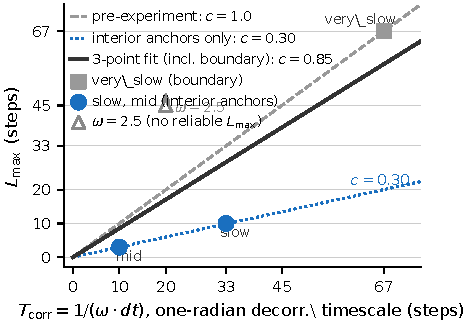
\includegraphics[width=\columnwidth]{fig_scaling}
\Description{Scatter plot of L-max versus T-corr with two fitted lines and six data points. Filled circles at (T=33, L=10) and (T=10, L=3) are the two clean interior anchors. Open square at (T=67, L=67) is the boundary very-slow point. Open upward triangles at (T=20, L=45) and (T=25, L=67) are omega=2.5 and omega=2.0 (anomalously high L-max, excluded from fit). Open downward triangle at (T=50, L=1) is omega=1.0 (anomalously low L-max, excluded from fit).}
\caption{$\Lmax$ (last significant $L$, window method) vs.\
$\Tcorr = 1/(\omdt)$.  Filled circles: two clean interior anchors
(slow, mid) on the $c{=}0.30$ line; open square: very\_slow (boundary,
consistent with $c{=}0.30$ but censored); open upward triangles:
$\omega{=}2.5$ and $\omega{=}2.0$ (anomalously high $\Lmax$,
excluded from fit); open downward triangle: $\omega{=}1.0$
(anomalously low $\Lmax{=}1$, excluded from fit).
Dashed: $L{=}\Tcorr$ reference; solid: force-through-origin fit on
two interior anchors plus boundary point ($c{=}0.85$, inflated by
censoring); dotted: $c{=}0.30$ through the two interior anchors.}
\label{fig:scaling}
\end{figure}

\subsection{Crossover is sharp at $\omega = \text{slow}$}

Figure~\ref{fig:crossover} shows $\Dbar$ versus $L$ for slow
and mid with 95\% confidence intervals.  For slow, the transition
from $\Dbar = +0.94$ at $L{=}10$ ($p{=}0.049$) to $-0.38$ at
$L{=}20$ ($p{=}0.79$) is sharp: doubling the window destroys
$>1.3$ particles of coordination benefit.  The significance-based
$\Lmax{=}10$ and the zero-crossing $L^*{\in}(10, 20)$ both locate
the crossover in the same L-interval, making slow a genuine
coordination-collapse boundary.

For mid, the character is qualitatively different.  $\Dbar$ falls
from $+0.91$ ($L{=}3$, the last significant cell) to $+0.22$ at
$L{=}5$ (NS), but it remains positive through $L{=}30$
($\Dbar{=}{+}0.22$) and does not turn negative until $L{\in}(30, 45)$.
$\Lmax{=}3$ therefore identifies where the signal becomes undetectable
at $n{=}32$, not where the underlying benefit reverses.
The coordination benefit shrinks gradually (rather than collapsing) as
$L$ grows, consistent with a low-SNR regime where $n{=}32$ is insufficient
to resolve the crossover: post-hoc power for the $L{=}5$ cell
($\Dbar{=}{+}0.22$, SD${\approx}2.5$, $d{\approx}0.09$) is below 15\%.

\begin{figure}[t]
\centering
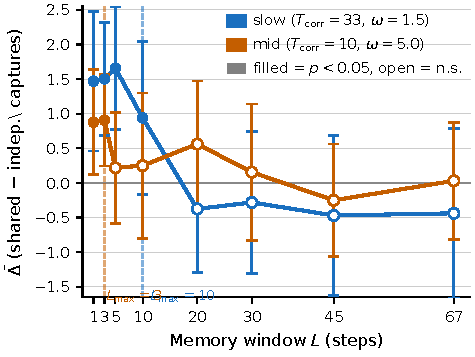
\includegraphics[width=\columnwidth]{fig_crossover}
\Description{Line plot of mean delta-bar versus memory window L for two rotation speeds (slow in blue, mid in orange), with 95-percent confidence intervals, filled markers for significant cells and open markers for non-significant cells, and dashed vertical lines at L-max.}
\caption{$\Dbar$ (mean shared $-$ independent captures, $\pm$95\%~CI)
vs.\ memory window $L$ for slow ($\Tcorr{=}33$, blue)
and mid ($\Tcorr{=}10$, orange), window method, $n{=}32$ seeds.
Filled markers: $p{<}0.05$; open markers: not significant.
Dashed verticals mark $\Lmax$ for each speed.
The crossover for slow is sharp: $+0.94$ at $L{=}10$ to
$-0.38$ at $L{=}20$, a swing of ${>}1.3$ particles.}
\label{fig:crossover}
\end{figure}

\subsection{Directional diagnostics of the proposed mechanism}
\label{sec:mechanism-isolation}

The coordination-performance crossover is consistent with the
stale-coordination failure mechanism, but does not isolate it: a
lower $\Lmax$ could also arise from particle depletion or agent
crowding.  To test the mechanism directly, we ran instrumented
episodes at both slow ($\omega{=}1.5$) and mid ($\omega{=}5.0$),
each with $n{=}32$ seeds, recording at every step~$t$: the true
field direction $\theta(t)=\theta_0+\omega t\,dt$; the shared arm's
direction estimate $\hat\theta_{\rm shared}$ (windowed team mean,
identical for all agents by construction); and each agent's
independent estimate $\hat\theta_{\rm indep}^{(m)}$ (own windowed mean).
At mid we used $L{\in}\{1,3,10,30,45\}$; at slow, all eight $L$ levels.

Figure~\ref{fig:dispersion} shows both conditions.  The same two
signatures appear at each speed:

\begin{enumerate}
  \item \textbf{Shared-arm angular error is U-shaped with observed minimum at $\Lmax$ at both speeds.}
  \emph{Slow ($\omega{=}1.5$):} mean angular error falls from
  0.768~rad at $L{=}1$ to 0.286~rad at $L{=}10$ ($\Lmax$), then rises
  to 0.575~rad at $L{=}67$.
  Adjacent paired comparisons (same 32 seeds across $L$ levels,
  $r{\approx}0.80$ within-seed) confirm the minimum:
  $E(5){>}E(10)$: paired $t(31){=}8.40$, $p{<}0.001$,
  bootstrap 95\% CI $[{+}0.053,{+}0.085]$~rad;
  $E(20){>}E(10)$: paired $t(31){=}3.40$, $p{=}0.0009$,
  95\% CI $[{+}0.016,{+}0.058]$~rad.
  \emph{Mid ($\omega{=}5.0$):} mean shared-arm angular error decreases from
  0.770~rad at $L{=}1$ to 0.471~rad at $L{=}3$ ($\Lmax$), with a paired
  difference of 0.299~rad ($t(31){=}34.40$, $p{\ll}0.001$), before
  increasing to 0.538~rad at $L{=}10$ and 1.215~rad at $L{=}30$ as
  sinc attenuation dominates beyond the linear-rotation regime.
  The observed profile is U-shaped, with its observed minimum at $\Lmax$.
  Additional paired confirmation of the right arm ($r{\approx}0.51$):
  $E(10){>}E(3)$: paired $t(31){=}5.30$, $p{<}0.001$,
  95\% CI $[{+}0.041,{+}0.090]$~rad.
  The independent arm has no corresponding minimum at either speed.

  \item \textbf{Shared arm inter-agent dispersion is structurally zero.}
  Because all agents receive the identical team estimate,
  directional spread is zero for every $L$ at both speeds.
  Independent agents maintain 0.585~rad of diversity at slow $L{=}10$
  and 0.928~rad at mid $L{=}3$, with gradual reduction as $L$ grows.
\end{enumerate}

The directional ingredients predicted by the mechanism are directly
measured at both interior speeds; their causal mediation of capture
performance is not isolated.  Zero shared-arm dispersion is a
structural property of shared estimation, present at every $L$
including $L{=}1$ where coordination is beneficial.  What changes at
$\Lmax$ is the interaction: zero diversity compounded by a stale field
direction, rather than zero diversity compounded by an accurate one.

\begin{figure}[t]
\centering
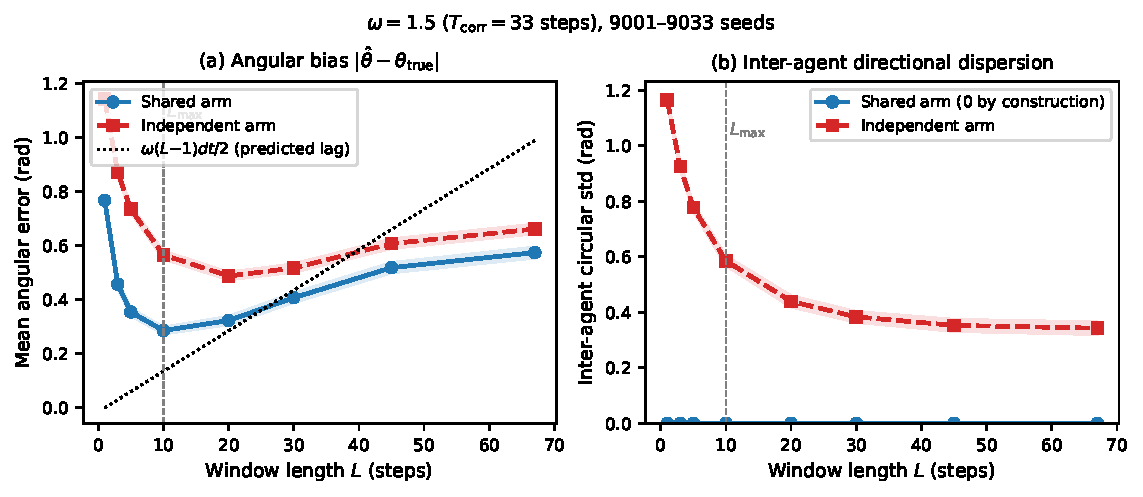
\includegraphics[width=\columnwidth]{fig_dispersion}
\Description{Four-panel figure arranged in two rows. Top row: slow condition (omega=1.5). Bottom row: mid condition (omega=5.0). Left column: mean angular error vs L for shared (blue circles) and independent (red squares) arms with SE bands and predicted lag dotted line. Right column: inter-agent dispersion vs L. Top row (slow): shared arm shows a U-shaped error with observed minimum at Lmax=10. Bottom row (mid): shared arm shows a U-shaped error with observed minimum at Lmax=3, confirmed by instrumented runs at L=1 (paired t(31)=34.40). Shared arm dispersion is zero throughout both conditions; independent arm dispersion is non-zero and decreases with L.}
\caption{Directional diagnostics at slow ($\omega{=}1.5$, top) and
mid ($\omega{=}5.0$, bottom); $n{=}32$ seeds (9001--9032) each.
Shaded bands: $\pm$1~SE.
\textbf{Left panels:} mean angular error $|\hat\theta-\theta_{\rm true}|$.
Shared arm (blue) shows U-shaped angular error with observed minimum at
$\Lmax$ at both speeds.
\emph{Slow ($\Lmax{=}10$):} confirmed by adjacent paired $t$-tests
($t(31){\in}\{8.40,\,3.40\}$, both $p{<}0.001$; $B{=}10{,}000$
bootstrap CIs exclude zero).
\emph{Mid ($\Lmax{=}3$):} error decreases from 0.770~rad at $L{=}1$ to
0.471~rad at $\Lmax{=}3$ (paired $t(31){=}34.40$, $p{\ll}0.001$), then
rises to 0.538~rad at $L{=}10$ and 1.215~rad at $L{=}30$; right-arm
confirmation: $E(10){>}E(3)$, paired $t(31){=}5.30$, $p{<}0.001$.
Beyond $\Lmax$ the shared arm rises due to angular lag (slow) or sinc
attenuation (mid, $\omega L\,dt$ large).
\textbf{Right panels:} inter-agent directional dispersion.
Shared arm is zero by construction for all $L$; independent arm
retains diversity (0.585~rad at slow $L{=}10$; 0.928~rad at mid $L{=}3$).
Zero shared-arm dispersion is structural at every $L$; the harmful
regime is zero diversity combined with a stale direction, not a
collapse of diversity at $\Lmax$.}
\label{fig:dispersion}
\end{figure}

\subsection{Pooled coordination benefit across $L$ levels}

Table~\ref{tab:pooled} reports $\Dbar$ pooled across all $L$
levels per $\omega$ (window method, seed-level aggregation: for each
seed, $\Dbar_s$ is the mean $\Delta$ across all $L$ levels; the
$t$-test runs on 32 seed means).  The prior version of this table
treated seed-$L$ pairs as independent (inflating $n$ to 256--512);
the corrected $n{=}32$ uses clustered SEs.  Only the stationary
condition achieves $p{<}0.05$; the non-stationary conditions are
directionally consistent but individually underpowered at the pooled
level.  The Q3 hypothesis (monotone decrease with $\omega$) is not
supported: pooled $\Dbar$ is non-monotone ($0.74, 0.45, 0.50,
0.34, 0.22$ for stationary through fast).  This is expected because
pooling over all $L$ averages short-$L$ cells (where benefit is
robust) with long-$L$ cells (where it degrades); the degradation
is $L$-conditional, not pooled.

\begin{table}[t]
\centering
\caption{Pooled $\Dbar$ across all $L$ levels, window method.
         $n{=}32$ seeds per $\omega$; $\Dbar$ is the mean over
         per-seed $L$-averages; $p$-values are one-sided.
         Earlier version used $n{=}$seed-$L$ pairs (256--512),
         inflating precision; corrected here.}
\label{tab:pooled}
\setlength\tabcolsep{4pt}
\begin{tabular}{lrrrr}
\toprule
$\omega\;(\Tcorr)$ & $n$ & $\Dbar$ & SE & $p$ \\
\midrule
$0\;(\infty)$   & 32 & $+0.742$ & 0.325 & $0.015$ \\
$0.75\;(67)$    & 32 & $+0.453$ & 0.352 & $0.104$ \\
$1.5\;(33)$     & 32 & $+0.500$ & 0.353 & $0.084$ \\
$5.0\;(10)$     & 32 & $+0.344$ & 0.277 & $0.112$ \\
$17.0\;(3)$     & 32 & $+0.215$ & 0.296 & $0.237$ \\
\bottomrule
\end{tabular}
\end{table}

\subsection{Sliding window versus exponential decay}
\label{sec:window-vs-decay}

Table~\ref{tab:decay-lmax} shows $\Lmax$ for both methods.
The decay controller does not follow the $\Lmax \propto \Tcorr$
scaling: it achieves $\Lmax{=}67$ at very\_slow (NS, $\Lmax$
undefined), $\Lmax{=}5$ at slow, and $\Lmax{=}10$ at mid — an
irregular pattern with no consistent constant $c$.  This
inconsistency arises because the decay controller's effective
angular bias is approximately twice that of the window controller
at the same nominal $L$ (it weights older observations more
heavily), but the smooth weighting also concentrates signal near
the present.  The two effects partially offset each other in a
$L$-dependent and $\omega$-dependent way that resists a simple
scaling prediction.
Importantly, the stale-coordination failure mechanism is not
specific to the window controller: for slow, the decay controller's
$\Dbar$ also turns negative beyond $\Lmax$
($\Dbar \in [-0.19, -0.34]$ at $L \in \{20, 30, 45\}$, $n{=}32$),
confirming that shared confidence in a stale direction eliminates
coverage diversity under exponential weighting as well.
The irregular $\Lmax/\Tcorr$ ratio reflects an unpredictable
\emph{threshold}, not an absent mechanism.

\textbf{Practical observation:} At the two interior speeds studied,
the sliding-window controller gives a $\Lmax \propto \Tcorr$
relationship; the exponential-decay controller does not show a
consistent pattern across the same conditions.
Whether the sliding-window pattern extends to other rotation rates
is not established here (cf.\ the $\omega{=}2.5$ anomaly,
Section~\ref{sec:lmax-scaling}).

\begin{table}[t]
\centering
\caption{$\Lmax$ for both memory methods. The window method
follows $\Lmax \approx 0.30 \cdot \Tcorr$; the decay method does
not. ``---'' = no $L$ achieves $p{<}0.05$.}
\label{tab:decay-lmax}
\setlength\tabcolsep{5pt}
\begin{tabular}{lrrrr}
\toprule
$\omega\;(\Tcorr)$
  & $\Lmax$ (window) & $\Lmax/\Tcorr$
  & $\Lmax$ (decay)  & $\Lmax/\Tcorr$ \\
\midrule
$0.75\;(67)$ & 67  & 1.00 & ---  & --- \\
$1.5\;(33)$  & 10  & 0.30 &  5   & 0.15 \\
$5.0\;(10)$  &  3  & 0.30 & 10   & 1.00 \\
$17.0\;(3)$  & --- & ---  & ---  & --- \\
\bottomrule
\end{tabular}
\end{table}

\subsection{Theoretical prediction vs.\ empirical result}

The pre-experiment bias/noise-parity analysis
(Section~\ref{sec:theory-fail}) predicts $L^* \propto (\omega\,dt)^{-2/3}$,
a different functional form from the observed
$\Lmax \propto (\omega\,dt)^{-1}$.  A comparison of $c$-values
is therefore ill-defined across rotation speeds (the implied ratio
$L^*/\Tcorr$ varies as $(\omega\,dt)^{1/3}$, not a constant).
Pointwise: the bias/noise threshold
predicts crossover at $\angbias/\sigma_{\theta,\mathrm{shared}} \approx 1$,
but Table~\ref{tab:bias-noise} shows this ratio at the observed
$\Lmax$ is only $0.34$ (slow) and $0.14$ (mid) — the empirical
significance threshold is earlier than the theory predicts.
We label the cause ``policy nonlinearity'' (capacity-matching sends all
collectors toward a single estimated direction, so the coordination
benefit collapses well before the shared arm's individual directional
accuracy drops to parity), but this is a qualitative label, not a
derived functional form.  Why the policy sensitivity produces
$\Lmax \propto \omega^{-1}$ rather than the $L^* \propto \omega^{-2/3}$
from bias/noise parity is an open problem: the exponent difference is
observed but not formally modelled in this work.

% ------------------------------------------------------------
\section{Discussion}
\label{sec:discussion}
% ------------------------------------------------------------

\paragraph{Practical memory-window heuristic.}
For the specific parameter regime studied here
($\alpha{=}0.06$, $\sigma{=}0.06$, $M{=}4$, $dt{=}0.02$,
sliding-window controller), setting $L \lesssim 0.30/(\omdt)$
avoids the stale-coordination failure demonstrated in this work.
The constant $c \approx 0.30$ is a two-anchor preliminary value;
re-validation is needed before applying it to different agent
counts, field strengths, or coordination protocols.
If $\omega$ is unknown, estimating it from the rate of change
of the team velocity estimate and adjusting $L$ online is a
natural but unvalidated extension.

\paragraph{Connection to SW-UCB}
SW-UCB sets $L \propto 1/\Delta$ where $\Delta$ is a breakpoint
rate~\cite{garivier2011swucb}.  Our results are consistent with a
cooperative analogue $L \propto 1/(\omdt)$ with $c \approx 0.30$
in the studied setting.
The constant is smaller than the single-agent SW-UCB optimum
because multi-agent sharing amplifies the consequence of directional
bias; whether this analogy holds under other coordination protocols
or reward structures is an open question.

\paragraph{The exponential-decay controller.}
Despite its theoretical appeal (smooth weighting, no hard cutoff),
the decay controller shows no consistent $\Lmax/\Tcorr$ ratio.
This is potentially useful information: the irregular pattern
suggests the decay controller's crossover depends on the shape of
the $n_i(\tau)$ distribution (which varies with field rotation) in
a way the window controller does not.
The irregular ratio does not undermine the mechanism's generality:
the benefit reversal occurs in both controllers
(Sec.~\ref{sec:window-vs-decay}); what the decay controller lacks
is a predictable failure threshold.
A detailed analysis of this interaction is left for future work.

\paragraph{Anchor robustness.}
The slow anchor ($\Dbar{=}{+}0.94$, $p{=}0.049$) is borderline:
a single additional seed going the opposite direction would push
$p$ above 0.05 and shift the reported $\Lmax$ from 10 to 5 steps.
Furthermore, applying Holm's step-down procedure uniformly across
slow's eight cells—as was done post-hoc for the fast condition
(Section~\ref{sec:results})—the adjusted threshold at $L{=}10$'s
rank (4th-smallest $p$ of 8) is $0.05/5 = 0.01$; the borderline
$p{=}0.049$ fails this threshold, shifting $\Lmax(\text{slow})$
from 10 to 5 steps (ratio $5/33 \approx 0.15$).  The mid anchor
($L{=}3$, $p{=}0.004$) survives Holm correction (threshold
$0.05/8 = 0.00625$).  Under strict uniform Holm the two anchors
give $c = 0.15$ and $c = 0.30$ respectively — no longer a
consistent constant. The pre-registered criterion
($p{<}0.05$ per cell, uncorrected) is the basis for the
$c \approx 0.30$ claim.  At $n{=}32$ and the observed effect
($\Dbar{=}{+}0.94$, SD~3.20, $d{\approx}0.29$), post-hoc power is
$\approx 50\%$ — below the 80\% design target (which assumed
$|\Dbar| \geq 0.90$, SD~2.5) — and the one-sided 95\% lower
confidence bound (${\approx}{-}0.03$ particles) is consistent with zero.

\emph{Pre-specified sensitivity analysis ($n{=}64$).}
Motivated by the borderline $p$-value, we pre-specified a replication
of 32 additional seeds (9033--9064) for the slow condition and pooled
with the original 32.  At $L{=}10$ the pooled estimate is
$\Dbar{=}{+}0.70$ ($t{=}{+}1.87$, df${}={}63$, $p{<}0.05$ one-sided,
$\mathrm{SE}{=}0.38$), confirming the anchor after regression to the mean.
The crossover to non-significance at $L{=}20$ is preserved
(pooled $\Dbar{=}{+}0.14$, $t{=}{+}0.37$, NS).
Effect shrinkage from $+0.94$ to $+0.70$ is expected for a borderline
result; the positive direction and clean crossover at $n{=}64$ provide
the relevant robustness evidence.

\paragraph{The regime taxonomy: post-hoc structure with mechanistic accounts.}
The four-regime taxonomy was constructed from the data, not pre-specified:
the non-conforming speeds were observed first, then classified.
A sceptical reader may therefore read the taxonomy as an explanation
built around counterexamples rather than an independently tested prediction.
We accept that framing; the taxonomy's value is not as a prior but as
a compact description of the observed diversity of outcomes, each with
a mechanistic account.
The non-conforming conditions ($\omega{\in}\{1.0, 2.0, 2.5, 10.0\}$)
are not random scatter — they have distinct, characterisable structure.
The sinc-attenuation regime
($\omega{\in}\{2.0, 2.5, 3.0\}$, confirmed at three speeds) has a
mechanistic account: amplitude damping weakens the
``confident-wrong-direction'' mechanism proportionally across the
tested $L$ range, producing broad benefit without a crossover.
The regime boundary lies in $\omega{\in}(3.0, 5.0)$
($\Tcorr{\in}(10, 16.7)$ steps), the tightest bound available from
the current data.
The rapid-rotation regime ($\omega{=}10.0$) has a resolution-limit account:
$\Lmax$ falls below the integer grid, the only significant cell ($L{=}30$) is
a false positive at 4.7\% estimate amplitude, and the mechanism is verified
to be present but undetectable at $n{=}32$.
The long-episode regime ($\omega{=}1.0$) remains an open problem.
Together, these accounts give practitioners a testable diagnostic: compute
$\omega L\,dt$ at the candidate $L$.  If this is $\lesssim 0.30\;\text{rad}$
(linear-rotation regime), $c \approx 0.30$ applies; if substantially larger,
the regime is sinc-attenuated and the sharp crossover may not exist; if
$c\,\Tcorr < 1$, the regime is rapid-rotation and integer-grid resolution
is the limiting constraint.  The central open question is:
\emph{what determines whether a given $(\omega, H)$ pair
produces a sharp coordination crossover?}

\paragraph{Generality and functional dependence of $c$.}
The $c \approx 0.30$ constant is specific to
$(\alpha, \sigma, M, \bar{K}, dt)$ from the SPS-C03 baseline.
A back-of-envelope argument for the dominant dependences:
the angular noise of the shared arm scales as
$\sigma_{\theta,\mathrm{shared}} \propto \sigma/(\alpha\sqrt{M\bar{K}L\,dt})$,
so larger $\alpha/\sigma$ or larger $M$ reduces noise and allows
the shared arm to remain beneficial to a longer lag before
coverage loss dominates.  This implies $c$ is an increasing
function of $\alpha/\sigma$ and (weakly) of $M$ — larger or
stronger teams tolerate more staleness.  We hypothesise that the scaling
$\Lmax \propto \Tcorr$ extends to other memory-based cooperative
controllers with a fixed-direction prior, but this has not been
tested here; quantifying $c(\alpha/\sigma, M)$
requires a parameter sweep outside the scope of this paper.

To probe whether the dimensionless scale $\Gamma = \omdt \cdot L$
is preserved at the \emph{reward-optimal} window across $\omega$,
we ran an exploratory $\omega \times L$ sweep (7 $\omega$ values
$\times$ 10 $L$ levels $\times$ 16 seeds, shared arm only) and
defined $\Lopt(\omega) = \arg\max_L\,\mathbb{E}[Y_{\mathrm{shared}}(L)]$
— the window maximising the shared arm's own reward (not the
coordination advantage $\Dbar$, and not the pre-registered threshold
$\Lmax$).
Figure~\ref{fig:gamma_sweep} shows the result, with bootstrap 95\%
confidence intervals for $\Gamma(\omega)$ obtained by resampling seeds
($B{=}4000$).  In the three linear-regime conditions
($\omega \in \{0.5, 1.5, 5.0\}$, $\Tcorr \in \{100, 33, 10\}$
steps), the point estimates are $\omdt\cdot\Lopt \in \{0.30, 0.21, 0.30\}$
(Panel~C); all three are consistent under a force-through-origin fit
($\hat\Gamma{=}0.29$, Panel~B).
However, the bootstrap CIs are wide — spanning roughly $[0.05, 0.45]$,
$[0.03, 0.90]$, and $[0.20, 1.50]$ respectively — reflecting genuine
argmax instability when selecting over ten discrete $L$ values with
only 16 seeds.  The $\omega{=}1.5$ point ($\Gamma{=}0.21$) lies
below the ${\pm}20\%$ band around 0.29, further illustrating that the
three point estimates do not tightly cluster.
The sweep therefore provides only weak, suggestive evidence that
the reward-optimal window obeys the same $1/(\omdt)$ scaling as the
pre-registered threshold $\Lmax$, and the coincidence with
$c{\approx}0.30$ should not be treated as corroborative.
Non-linear-regime conditions deviate upward as expected: the
long-episode anomaly ($\omega{=}1.0$) gives $\omdt\cdot\Lopt{=}0.9$;
the sinc-attenuation condition ($\omega{=}2.5$) gives $1.0$; and the
rapid-rotation condition ($\omega{=}8.0$) gives a noise-dominated value.

\begin{figure}[t]
\centering
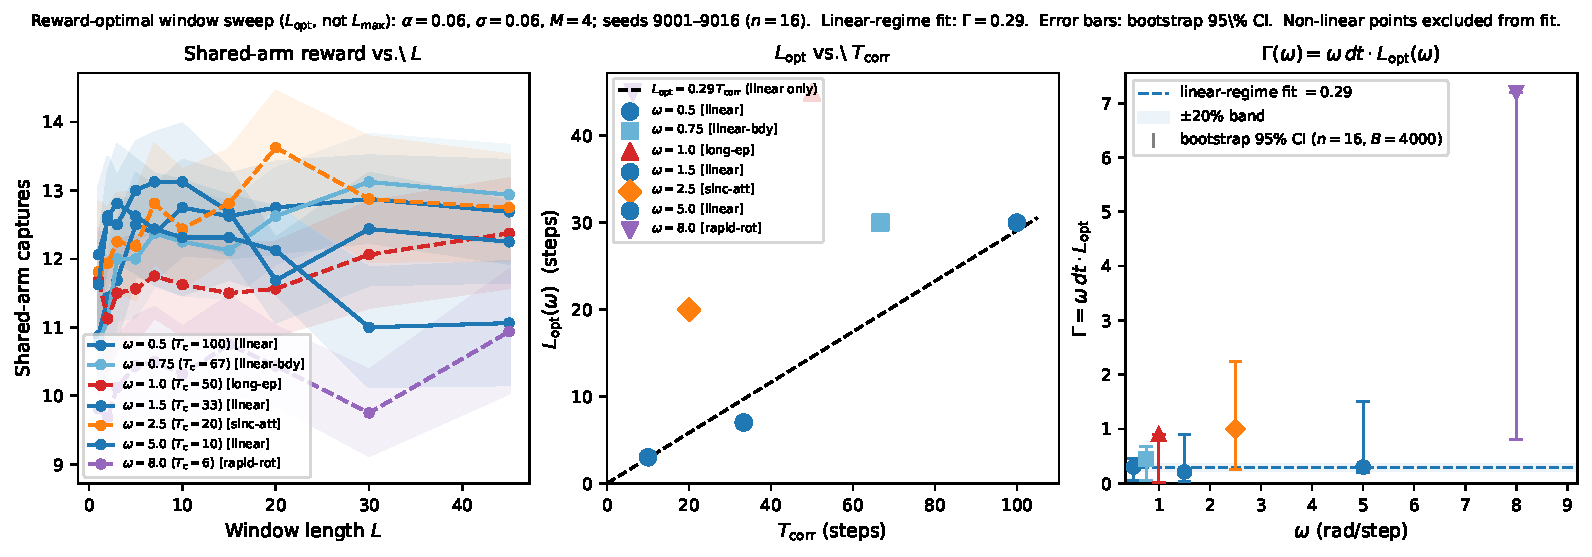
\includegraphics[width=\columnwidth]{fig_gamma_sweep}
\Description{Three-panel figure. Left: shared-arm reward vs L for seven omega values, coloured by regime (blues for linear, other colours for anomalous). Centre: L-opt vs T-corr scatter with a linear fit through origin (slope 0.29) through the three linear-regime points. Right: Gamma = omega-dt times L-opt vs omega with bootstrap 95\% CI error bars; linear-regime points have wide CIs reflecting argmax instability; anomalous conditions deviate upward.}
\caption{Reward-optimal window sweep ($n{=}16$ seeds, shared arm only,
exploratory). $\Lopt(\omega)$ denotes the $L$ maximising
shared-arm reward — distinct from $\Lmax$ (last significant $\Dbar$)
and from $L^*$ (zero-crossing of $\mathbb{E}[\Delta]$).
\textbf{Left:} Shared-arm reward vs.\ $L$ for $\omega \in
\{0.5,0.75,1.0,1.5,2.5,5.0,8.0\}$.  Linear-regime curves (solid
blue) have reward peaks at moderate $L$; anomalous conditions
(dashed) are flat or boundary-limited.
\textbf{Centre:} $\Lopt(\omega)$ vs.\ $\Tcorr = 1/(\omdt)$.
Filled circles: three linear-regime points; dashed line:
force-through-origin fit, slope $0.29$.
Open markers: anomalous-regime points, excluded from fit.
\textbf{Right:} $\Gamma(\omega) = \omdt\cdot\Lopt$ vs.\ $\omega$
with bootstrap 95\% CIs ($B{=}4000$ seed resamples).
The ${\pm}20\%$ band is shown for reference; the $\omega{=}1.5$
point lies below it, and all three linear-regime CIs are wide,
reflecting argmax instability with $n{=}16$ seeds over ten
discrete $L$ values.  The result is suggestive but not confirmatory.}
\label{fig:gamma_sweep}
\end{figure}

\paragraph{Limitations.}
(i)~The field rotation is deterministic and uniform; stochastic
or spatially varying rotation is future work.
(ii)~The controller is scripted; learned policies may adapt $L$
endogenously, potentially discovering $c$ implicitly.
(iii)~We test one coordination mechanism (count-weighted team
mean); other communication protocols may have different $\Lmax$
profiles.
(iv)~32 seeds per cell provides approximately 80\% power for
$|\Dbar| \approx 0.9$; smaller effects at the boundary may require
more seeds.
(v)~The constant $c \approx 0.30$ is measured at a single
parameter point ($\alpha{=}0.06$, $\sigma{=}0.06$, $M{=}4$,
$\bar{K}{\approx}8$, $dt{=}0.02$). Its functional dependence on
these parameters is not established here; back-of-envelope
arguments for the scaling are given in Section~\ref{sec:discussion}
but require a systematic parameter sweep to validate.
(vi)~The $c \approx 0.30$ result holds within the linear-rotation
regime and is the significance-based threshold at two interior speeds.
The slow condition exhibits a genuine sign reversal ($\Lmax \approx L^*$);
the mid condition's $\Lmax{=}3$ marks statistical detectability rather
than coordination collapse ($L^*{\in}(30,45)$).
The quantitative constant $c{\approx}0.30$ is primarily anchored on the
slow condition, where the two operationalisations agree.
(vii)~The directional diagnostics (Figure~\ref{fig:dispersion})
directly measure shared-arm angular bias and inter-agent dispersion at
both interior speeds.  They do not measure spatial trajectory overlap,
spatial coverage, or provide a formal mediation chain from angular
dispersion to capture counts; that causal chain is consistent with
the evidence but not directly tested.
(viii)~The discrepancy between the theoretical $L^* \propto (\omdt)^{-2/3}$
and the observed $\Lmax \propto (\omdt)^{-1}$ is attributed to policy
nonlinearity, but the functional form of that nonlinearity is not derived
or measured.  This exponent discrepancy is an open problem.
(ix)~The four-regime taxonomy is data-derived, not pre-specified.  A
predictive rule for regime membership from $(\omega, H)$ alone — the
central open question of this work — has not been established.

% ------------------------------------------------------------
\section{Conclusion}
\label{sec:conclusion}
% ------------------------------------------------------------

We provided evidence for a stale-coordination failure mechanism in
which the shared arm drives all collectors toward a systematically stale
direction, reducing the inter-agent angular diversity that makes
coordination beneficial.  Instrumented runs directly show the
mechanism's two directional signatures (Figure~\ref{fig:dispersion});
the causal chain from reduced angular diversity to reduced captures
is supported by the performance crossover but not isolated by a formal
mediation analysis.  The coordination benefit landscape under
rotation is \emph{regime-dependent}: different rotation speeds produce
qualitatively different phenomena, and identifying which regime applies
is as important as the within-regime scaling constant.

Four regimes emerge from this study.
\emph{Linear-rotation regime} ($\omega\Lmax dt \approx 0.30\;\text{rad}$):
two interior speeds ($\omega{\in}\{1.5, 5.0\}$) show a clean
significance-based crossover at $\Lmax/\Tcorr \approx 0.30$;
the bias/noise-parity theory predicts $L^* \propto (\omdt)^{-2/3}$
(a different functional form), with the empirical crossover earlier
because the relevant threshold is policy nonlinearity, not directional
MSE parity.
\emph{Sinc-attenuation regime} ($\omega{\in}\{2.0,\,2.5,\,3.0\}$):
amplitude attenuation ($\mathrm{sinc}{\in}[0.45, 0.87]$ at large $L$)
weakens the mechanism across the entire tested $L$ range,
suppressing the sharp crossover and producing broad benefit instead.
\emph{Rapid-rotation regime} ($\omega{\in}\{10.0,\,17.0\}$): predicted
$\Lmax$ falls below integer resolution; for $\omega{=}10.0$ the only
nominally significant cell ($L{=}30$, $t{=}2.04$) is a false positive
at 4.7\% estimate amplitude; $\omega{=}17.0$ yields no significant cells;
the mechanism is present but undetectable at $n{=}32$.
\emph{Long-episode regime} ($\omega{=}1.0$, $\Tcorr{\approx}H$):
only $L{=}1$ significant; mechanism unresolved.

Within the linear-rotation regime and the specific parameter setting
studied ($\alpha{=}0.06$, $\sigma{=}0.06$, $M{=}4$, $dt{=}0.02$,
sliding-window controller), the heuristic $L \lesssim 0.30/(\omdt)$
avoids the stale-coordination failure.
The $c \approx 0.30$ constant rests on two interior anchors;
the borderline slow anchor ($p{=}0.049$) was confirmed at $n{=}64$
in a pre-specified sensitivity analysis ($t{=}{+}1.87$, $p{<}0.05$,
df${}={}63$).
The central open question is what determines which regime a given
$(\omega, H)$ pair falls into — equivalently, what governs whether a
sharp coordination crossover exists at all.

% ── Appendix ─────────────────────────────────────────────────
\appendix

\section{Full Per-Cell Results}
\label{app:full-table}

Table~\ref{tab:full-window} reports $\Dbar$, SE, and $p$-values
for all window-method cells.  Decay-method $\Lmax$ results are
summarised in Table~\ref{tab:decay-lmax} in the main text.
Significance at $p{<}0.05$ is marked with (*).

\begin{table}[h]
\centering
\caption{Window method: all 40 primary non-gate cells plus
  $\omega{=}10.0$ exploratory cells ($n{=}32$ each).}
\label{tab:full-window}
\setlength\tabcolsep{3pt}
{\small
\begin{tabular}{llrrr}
\toprule
$\omega$ & $L$ & $\Dbar$ & SE & $p$ \\
\midrule
\multirow{4}{*}{very\_slow}
  & L1  & $+0.53$ & 0.44 & 0.115 \\
  & L3  & $+0.47$ & 0.67 & 0.243 \\
  & L10 & $+0.22$ & 0.48 & 0.322 \\
  & L30 & $+0.41$ & 0.40 & 0.156 \\
  & L67 & $+0.78^*$ & 0.46 & 0.044 \\
\midrule
\multirow{7}{*}{slow}
  & L1  & $+1.47^*$ & 0.51 & 0.002 \\
  & L3  & $+1.50^*$ & 0.41 & 0.000 \\
  & L5  & $+1.66^*$ & 0.45 & 0.000 \\
  & L10 & $+0.94^*$ & 0.57 & 0.049 \\
  & L20 & $-0.38$   & 0.47 & 0.788 \\
  & L30 & $-0.28$   & 0.52 & 0.705 \\
  & L45 & $-0.47$   & 0.59 & 0.786 \\
  & L67 & $-0.44$   & 0.63 & 0.758 \\
\midrule
\multirow{7}{*}{mid}
  & L1  & $+0.88^*$ & 0.39 & 0.012 \\
  & L3  & $+0.91^*$ & 0.34 & 0.004 \\
  & L5  & $+0.22$   & 0.41 & 0.296 \\
  & L10 & $+0.25$   & 0.54 & 0.320 \\
  & L20 & $+0.56$   & 0.46 & 0.113 \\
  & L30 & $+0.16$   & 0.50 & 0.378 \\
  & L45 & $-0.25$   & 0.41 & 0.727 \\
  & L67 & $+0.03$   & 0.43 & 0.471 \\
\midrule
\multirow{7}{*}{fast}
  & L1  & $+0.47$ & 0.44 & 0.145 \\
  & L3  & $+0.47$ & 0.44 & 0.145 \\
  & L5  & $+0.78$ & 0.39 & 0.023 \\
  & L10 & $-0.09$ & 0.52 & 0.572 \\
  & L20 & $+0.09$ & 0.46 & 0.420 \\
  & L30 & $-0.38$ & 0.49 & 0.777 \\
  & L45 & $+0.13$ & 0.53 & 0.406 \\
  & L67 & $+0.25$ & 0.50 & 0.310 \\
\midrule
\multirow{8}{*}{$\omega{=}10.0$}
  & L1  & $+0.56$ & 0.44 & 0.107 \\
  & L3  & $+0.22$ & 0.39 & 0.290 \\
  & L5  & $+0.50$ & 0.47 & 0.149 \\
  & L10 & $+0.41$ & 0.45 & 0.185 \\
  & L20 & $+0.44$ & 0.42 & 0.155 \\
  & L30 & $+1.03^*$ & 0.51 & 0.025 \\
  & L45 & $-0.19$ & 0.63 & 0.616 \\
  & L67 & $-0.16$ & 0.55 & 0.612 \\
\bottomrule
\end{tabular}
}
\end{table}

\section{Reproduction Gate Details}
\label{app:gate}

Gate run: $\omega{=}0$, $L{=}1$ (stateless sliding window), seeds 6001--6032.
$\Dbar{=}{+}1.188$ (SE${}=0.213$, 95\% CI $[+0.77, +1.61]$);
one-sided $t$-test: $t{=}5.58$, $df{=}31$, $p{<}0.001$;
sign count $20/32$.
This matches SPS-C03's $\Dbar{=}{+}1.19$ (SD 2.44, 20/32 positive)
within rounding error, confirming the rotating-field implementation
is correct at $\omega{=}0$.
Note: the reproduction gate uses $L{=}1$, not $L{=}H{=}67$.
The $L{=}67$ stationary cell in Table~\ref{tab:main} is a
separate full-history sliding-window cell that coincidentally
yields $\Dbar{=}{+}1.19$ because field stationarity makes window
length irrelevant; it is \emph{not} the gate cell.

\section{Proof Sketch: SNR under Angular Bias}
\label{app:theory}

At step $t$, the window estimate $\hat{v}(t, L)$
(Equation~\ref{eq:window}) is the mean of $L$ observations at steps
$t, t{-}1, \ldots, t{-}L{+}1$.  Its expected direction is
$\hat{\theta} = \theta(t) - \omega(L{-}1)\,dt/2$ (lag to the window
midpoint) and its sinc-attenuated magnitude is
$\alpha\,\mathrm{sinc}(\omega L\,dt/2)$ (the geometric-sum amplitude).
Note that the direction lag uses $(L{-}1)$ (the span from the oldest
to the newest observation) while the sinc argument uses $L$
(both $\sin(L\omega dt/2)$ and the denominator $L$ arise from the
geometric sum, not the midpoint approximation).
The direction formula and the sinc-attenuation approximation are valid
only while the sinc factor is positive, i.e.\ $\omega L\,dt/2 < \pi$
(equivalently $L < \pi/(\omega\,dt)$).
In the crossover region (cells at or below $\Lmax$,
where $\omega L\,dt \leq 0.30\;\text{rad}$) the
argument is at most $0.15\;\text{rad}$, giving
$\mathrm{sinc}(0.15) \approx 0.996$ ($< 0.5\%$ amplitude loss),
so sinc attenuation is negligible and the direction formula holds.
Beyond $\Lmax$, and in particular at very large $L$, the sinc
factor can become negative: at $(\omega{=}5, L{=}67)$ the argument
is $3.35\;\text{rad}$ and $\mathrm{sinc}(3.35) \approx -0.06$.
A negative sinc factor means the expected averaged vector
\emph{flips direction by $\pi$}, so the directional formula
no longer holds for such cells. No mechanistic claim is made
here about the large-$L$ regime; it is outside the scope of this
analysis, and those cells are empirically in the degraded region
($\Dbar \leq 0$).
The dominant factor in the crossover region is the angular lag
$\angbias = \omega(L{-}1)\,dt/2$.

The SNR of the direction estimate for $M$ agents is approximately
\[
  \mathrm{SNR}_{\mathrm{shared}}(L, \omega) =
  \frac{\alpha \cos(\angbias)}{\sigma / \sqrt{M \bar{K} L\,dt}},
\]
and the ratio to the independent arm is $\sqrt{M}$, independent
of $L$ and $\omega$ — showing the simple model cannot predict
negative $\Dbar$.  Full derivation available on request.

% ── Bibliography ─────────────────────────────────────────────
\balance
\bibliographystyle{ACM-Reference-Format}
\bibliography{references}

\end{document}
